\documentclass[12pt, letterpaper, oneside, notitlepage, onecolumn]{article}
\author{William Baskin}
\title{Dynamic Festo Model}
\pagestyle{plain}

\usepackage{parskip}

\usepackage{textcomp}
\usepackage[utf8]{inputenc}
\usepackage[english]{babel}
\usepackage{listings}
\usepackage{color}
\usepackage{verbatim}
% \usepackage{soul}
\usepackage[margin=0.69in]{geometry}

% math
\usepackage{amsmath, amssymb, amsthm}
% \usepackage{amsmath, amssymb, amsthm, gensymb}

\usepackage{graphicx}
% \graphicspath{ {graphics/} }
% \includegraphics[height=6.75in,angle=270]{HW25}

\definecolor{dkgreen}{rgb}{0,0.6,0}
\definecolor{gray}{rgb}{0.5,0.5,0.5}
\definecolor{mauve}{rgb}{0.58,0,0.82}

\lstset{frame=tb,
  language=Python,
  aboveskip=3mm,
  belowskip=3mm,
  showstringspaces=false,
  columns=flexible,
  basicstyle={\small\ttfamily},
  numbers=none,
  numberstyle=\tiny\color{gray},
  keywordstyle=\color{blue},
  commentstyle=\color{dkgreen},
  stringstyle=\color{mauve},
  breaklines=true,
  breakatwhitespace=true,
  tabsize=3
}

\DeclareMathOperator*{\argmax}{arg\,max}

\DeclareMathOperator*{\argmin}{arg\,min}

\newcommand{\subsubsubsection}{\paragraph}
\newcommand{\bbs}[1]{\section{#1}}
\newcommand{\bbss}[1]{\subsection{#1}}
\newcommand{\bbsss}[1]{\subsubsection{#1}}
\newcommand{\bbssss}[1]{\subsubsubsection{#1}}

\newcommand{\norm}[1]{\left\lVert#1\right\rVert}

\usepackage[pdftex,
    pdfusetitle
    ]{hyperref}

\begin{document}
\maketitle

\section{General Model}

The key components of the acceleration calculation are highlighted in green.

\begin{equation}
M \ddot{\theta} + C \dot{\theta} + N = \tau
\end{equation}

\begin{center}
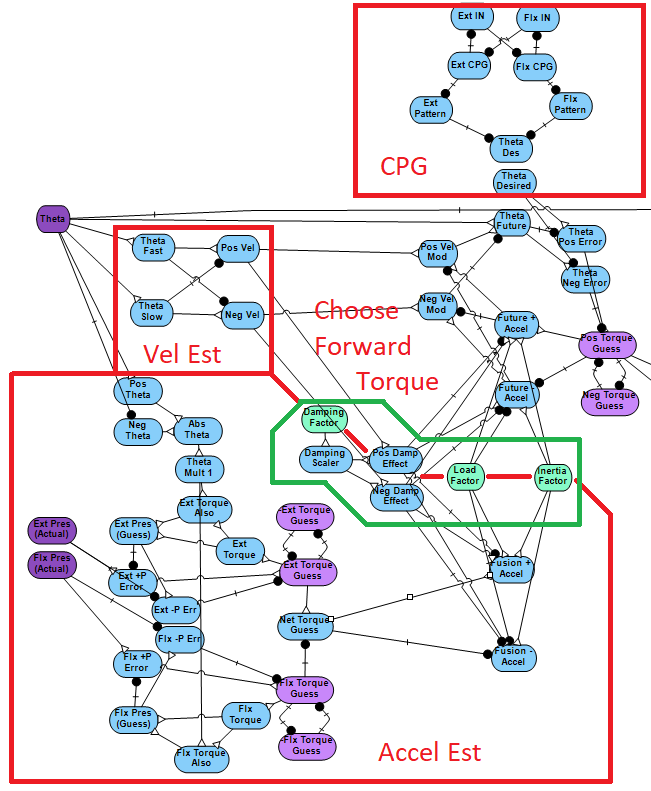
\includegraphics[height=5in, angle=0]{NetworkLayout}
\end{center}

The Inertia Factor (M) is connected via a division synapse. The Load Factor (N) is a signal transfer network. The Damping Factor (C) is connected via a multiplication synapse to modulate damping effects based on the sign of the velocity.

\end{document}
